\documentclass{report}
\usepackage[margin=2.5cm]{geometry}
\usepackage{amsmath, amssymb, stmaryrd, latexsym, amsthm, mathtools}
\usepackage{mathpazo, times}
\usepackage{float}
\usepackage{listings}
\usepackage{url}
\usepackage{natbib}
% \usepackage{parskip} % very ugly with lemmas, invariants, etc without intervening text
\usepackage[disable]{todonotes}
\usepackage{slashed}
\usepackage{tikz}
\usetikzlibrary{automata, positioning, arrows}
\tikzset{
    state/.style={
           rectangle,
           rounded corners,
           draw=black, very thick,
           minimum height=2em,
           inner sep=2pt,
           text centered,
           },
}

\usepackage{forest}
\usepackage{IEEEtrantools}
\usepackage{microtype}
\usepackage{graphicx,color}

\usepackage{hyperref}
\hypersetup{
  colorlinks=false,
  linkcolor={blue},
  citecolor={blue},
  urlcolor={blue},
  linkbordercolor={white},
  citebordercolor={white},
  urlbordercolor={white}
}
\usepackage[capitalise,noabbrev,nameinlink]{cleveref}

% https://tex.stackexchange.com/questions/132823/ieeetrantools-clash-with-cleveref
\makeatletter
\let\if@IEEEissubequation\iffalse
\makeatother

\usetikzlibrary{arrows}

\newcommand{\coot}[1]{\textcolor{violet}{\emph{#1}}}
\newcommand{\njd}[1]{\textcolor{purple}{\emph{#1}}}
\newcommand{\avieth}[1]{\textcolor{blue}{\emph{#1}}}
\newcommand{\dcoutts}[1]{\textcolor{orange}{\emph{#1}}}
\addtolength{\marginparwidth}{-0.1\marginparwidth}

\newcommand{\var}[1]{\mathit{#1}}
\newcommand{\type}[1]{\mathsf{#1}}
\newcommand{\powerset}[1]{\mathbb{P}(#1)}
\newcommand{\order}[1]{\mathcal{O}\left(#1\right)}
\newcommand{\restrictdom}{\lhd}
\newcommand{\subtractdom}{\mathbin{\slashed{\restrictdom}}}
\newcommand{\restrictrange}{\rhd}

\DeclareMathOperator{\dom}{dom}
\DeclareMathOperator{\range}{range}
\DeclareMathOperator*{\argmin}{arg\,min} % thin space, limits underneath in displays
\DeclareMathOperator*{\minimum}{min}
\DeclareMathOperator*{\maximum}{max}

% Number within sections, and don't have separate counters for separate environments
\theoremstyle{definition}{
  \newtheorem{lemma}{Lemma}[section] % Number within sections
  \newtheorem{definition}[lemma]{Definition}
}
\theoremstyle{theorem}{
  \newtheorem{invariant}[lemma]{Invariant}
  \newtheorem{proofobligation}[lemma]{Proof Obligation}
}

\Crefname{invariant}{Invariant}{Invariants}

\numberwithin{equation}{lemma}

%\floatstyle{boxed}
%\restylefloat{figure}

\lstset{basicstyle=\ttfamily\small}

\raggedbottom

\begin{document}

\title{Data Diffusion and Peer Networking in Shelly\\
       {\small (Version 0.1)} \\
       {\large \sc An IOHK technical report}}
\author{Duncan Coutts \\ {\small \texttt{duncan@well-typed.com}} \\
                         {\small \texttt{duncan.coutts@iohk.io}}
   \and Alex Vieth \\ {\small \texttt{alex@well-typed.com}}
   \and Neil Davies \\ {\small \texttt{neil.davies@pnsol.com}} \\
                       {\small \texttt{neil.davies@iohk.io}}
   \and Marcin Szamotulski \\ {\small \texttt{marcin.szamotulski@iohk.io}}
   \and Karl Knutsson \\ {\small \texttt{karl.knutsson@iohk.io}}
   \and Marc Fontaine \\ {\small \texttt{marc.fontaine@iohk.io}}
   }
\date{January 08 2019}

\maketitle

\begin{abstract}
  This document describes .....
\end{abstract}

\tableofcontents

\section*{Version history}

\begin{description}
\item[Version 0.1, Dez 20, 2018  Draft of the table of contents.]
\item[Version 0.1.1, Jan 08, 2019 Structure and outline]
\end{description}

\chapter{Overview}
\section{Context and Introduction}

How this work relates (in general terms) to the rest of the Shelly
development and the Ourbouros papers.

\subsection{Data Diffusion assumptions in Ourbouros}
\begin{quote}
  This is the ``telling them what you are going to tell them'' part -
  outline of the data diffusion and overlay network bringing out the
  key functional and non-functional relationships - aim to serve as a
  general executive overview as well as a framing of PoS issues.
\end{quote}
\begin{itemize}
  \item Assumptions of the mathematical model(s)
  \item Goal of the data diffusion functionality
  \item Strong requirement on collective performance
  \begin{itemize}
    \item Chain growth quality
    \item Adverserial actor assumption
  \end{itemize}
\end{itemize}
\subsection{Functional Layering}
pictures as to how the various functional layers relate; How the Data
diffustion layer relates to Ledger etc; How data diffusion relates to
point-to-point overlay network.

\subsubsection{Non-function aspects}
Performance; trustworthiness; Forwarding as an expression of confirmed
``trust'' (and corollary - forwarding of \emph{clearly} incorrect information
seen as prima-facia evidence of adversarial action.
\subsection{Protocol Roles}
Peer relationship between various nodes; Limited trust and
verification; (Brief) description of the expectations and assumptions across
the functionality boundaries; 

\subsubsection{Mini Protocols}
\begin{description}
\item[Chain Tip Following] (or whatever the agreed name is)
\item[Bulk Chain Download] ....
\item[Transaction Difussion] ....
\item[$\Delta Q$ Measurement] (not really an mini protocol, in that it
  is point to point and not part of the diffusion process itself,
  placed here because it ``sits'' on top of the overlay network. Role
  to generate active endpoint performance data to help optimise
  time-to-diffuse critical information exchanges (e.g. newly minted
  block diffusion)
\end{description}  
\subsubsection{Point to point Overlay Network}
need picture; note that long term eclipse attacks are not an issue
here (cover why a bit later); tie in chain growth requirements with
need for ``better'' communications performance between (major)
stakepools (notion of Core DIF); association explain need for
\begin{itemize}
\item fixed configuration (with/without others from this list)
\item Core DIF
\item Distributed endpoint discovery (subset of notion of peer in
  other approaches)
\end{itemize}

  
\section{Layout of the Document}

\begin{itemize}
  \item What goes in which section ?
  \item In which order to read ?
  \item Which sections can be skipped ?
\end{itemize}

\section{Notation}

\chapter{Requirements}

\section{Performance Requirements and User Stories}
\subsection{Classes of Participants}
todo: make a nice table
\subsubsection{Stake pool} % lookup what this is called in the protocols.tex
\subsubsection{Small stakeholder}
\subsubsection{User who has delegated}
\subsubsection{Requiremts for Participants}
\subsubsection{Requiremts for Stake Pools}
\subsubsection{Services that the System should provide}

There are two kinds of Requirements:

\begin{enumerate}
\item System capabilities for a node to take a blockchain slot creation role in the protocol.
\item What services that the system provides to the user.
\end{enumerate}



\section{Protocol Updates on the Blockchain}
\begin{itemize}
\item Hydrid phase of federation and decentralization
\item Gradually transition between protocol variants on a life blockchain.
\item Several protocol variant active in parallel.
\item Communication between Shelley Nodes and existing core nodes.
\end{itemize}

\section{Node to Node and Node to Consumer IPC}
There are two basic variants of inter-process-communication in the network:
\begin{itemize}
\item IPC between Cardano nodes that are engaged in the high level Ouroboros
      blockchain consensus protocol.
\item IPC between a Cardano node and a `chain consumer' component such as a
      wallet, explorer or other custom application.
\end{itemize}
Both variants of IPC in the network follow destinct requirements and contraints, and
,while the first version of Cardano used a single protocol, the new version will
use different sets of protocols for both uses cases.
(See Section \ref{why_distinguish_protocols} for the motivation for this design decision.)
Throughout the document it will be clear which variant of we are referening to.

\section{Threat Model}
Todo: find out what a threat model is and whether it should be part of this document.
\subsection{Resource Consumption Attacks}


\section{Ouroboros}

How PoS is different from PoW in its network requirements:

\begin{itemize}
  \item No capability to sustain an undetected Eclipse attack
  \item Sustained liveness requirement
\end{itemize}

\section{Delegation}

\chapter{System Architecture}
\section{Overview}

Traditionally network protocols are presented as a stack of layers where
upper layers build on services provided by lower layers and lower layers
are agnostic of the implementation of the upper layers.
This concept of layers is misleading when discussing Shelly.
It is {\em not} the case that the consensus (layer) is build on top of the network (layer).
It is more appropriate to talk about a network component than a network layer.
The network component provides services to the consensus component and also vice versa.
The network component uses the consensus component to carefully validate every piece of
information that it distributes to other nodes.
This is essential to guard against certain kinds of DoS attacks.
This is also the reason why the network component in Shelly cannot be replaced
with an of-the-shelf peer-to-peer protocol.

\section{Design Choices}
\begin{itemize}
\item Only the design choices that have been taken.
\item Design discussions in the discussions section.
\end{itemize}
\section{Nodes}
\subsection{Node Components}

\chapter{Infrastructure}
Specific assumptions about the infrastructure that are relevant for the discussion.

\section{Internet}
\section{Network Toplogy}
\section{Topographical distribution of block creating nodes}
\section{TCP}

\section{Operating Systems}
\section{Firewall}
\section{Nodes and Hosting}

\chapter{Protocols}
\section{Protocols as State-machines}
The reference implementation of serveral sub-protocols uses a generic framework
for state-machines.

A Haskell implementation of the state machine framework is described in Section
\ref{Haskell-state-machine}. It uses correct by construction techniques to guarantee
several properties of the protocol and the implementation.
In particular it guaratees that there are no deadlocks. At any time, one side has agency
(is expected to transmit the next message) and the other side is waiting for the message,
or both sides agree the the protocol has terminated.
The transmission of a message that is not expected by the protocol aborts the exectution
of the protocol.

For each sub-protocol that is based on this underlying framework, the description provides the
following pieces of information:

\begin{itemize}
\item An informal description of the protocol.
\item Who is communication.
\item States of the state-machine
\item The messages that are exchanged
\item A transition graph of the global view of the state machine.
\item A transition graph of the client view.
\item A transition graph of the server view.
\end{itemize}

\begin{description}
\item[State Machine]
  The Protocols are described as a state machine.
  The specification uses different representations of the state machine,
  for example transition tables or diagrams, that all describe the same protocol.

\item[States]
  We need to distinguish between the global state of a system,
  which includes the values of all local variable stored on the nodes,
  and the abstract states of the the state machines.
  The abstract states are equivalent classes of the global state.
  Every global state belongs to exactly one abstract state.
  This specification describes the state machine in terms of the abstract states.
  By definition, client and server are always in identical states
  which also means that client and server simultaneously transit to new states.
  The concrete implementation needs to relax the definition of state.
  In the concrete implementation the abstract view of state is replaced with
  client state and server state and transitions on either side happens independently
  when a message is send or received.
  While a message is in-flight the state of the receiver is undefined.
  The state determines which side is active the client or the server.
  
\item[Messages/Events]
  Messages are elements from the set
  $\{(lable, data) \mid lable \in Labels, data \in Data\}$.
  Protocols use a small set of $Lables$ typically $|Labels| \leq 10$.
  State-machine frame work requieres that messages can be serialized,
  transferred over the network and de-serialized by the receiver.
  The binary format for messages is described in Section \ref{CBOR-section}.
\item[Transitions]
  This part of the document describes the transitions of the abstract state of the protocol
  as the result of messages passed between client and the server.
  In sync with abstract state the  client and server update the local data to compute the
  the actual "outcome" of a protocol-run, for example "update the block chain".
  Parts of the local updates are specific to the implementation language and the underlying
  data structures, but they are also relevant for the protocol (to determine the next transition).
\end{description}

\section{Single Phase Chain Synchronization Protocol}
\subsubsection{Description}
\begin{description}
\item[purpose of the protocol]

The Chain Synchronization Protocol is used by the block chain consumer
to synchronize its block chain with the block chain producer.
It is polymorphic on blocks. And for some clients it will synchronize just headers (node-to-node),
for others it can be used to synchronize actual block (e.g., node-to-wallet).

\item[Who is communicating]
  A node communicates with several upstream and downstream node.
  The node runs an independent agents for every other node
  it communicates with. The typically a node runs agents where it acts as a server and also instances
  where it acts as a client.(See Figure \ref{chain-diagram-read-pointers}.)
\end{description}


\begin{description}
\item[purpose of the protocol]
The Chain Synchronization Protocol is used by the block chain consumer
to synchronize its block chain with the block chain producer.
\item[Who is communicating]
  A node communicates with several upstream and downstream node.
  The node runs an independent agents for every other node
  it communicates with. The typically a node runs agents where it acts as a server and also instances
  where it acts as a client.
\item[Where is located in the protocol stack ?]
\item[What are the interfaces to the lower layers of the stack ?]
  The chain synchronization protocol can send and receive messages. (via a point to point channel.)
\item[Initialization of an instance of the protocol]
\end{description}

\subsubsection{State machine}
\begin{figure}[H]
\begin{tabular}{|l|l|}
  \hline
  \multicolumn{2}{|c|}{States} \\ \hline
  Name  & Agency \\ \hline \hline
  Idle       & client \\ \hline
  CanAwait   & server \\ \hline
  MustReply  & server \\ \hline
  Intersect  & server \\ \hline
  Done       &        \\ \hline
  \hline
\end{tabular}
\end{figure}

\begin{figure}[H]
\begin{tabular}{|l|l|l|l|}
  \hline
  \multicolumn{4}{|c|}{Transitions} \\ \hline
  message/event      & parameter              & from        & to       \\ \hline\hline
  RequestNext        &                        & Idle        & CanAwait \\ \hline
  AwaitReply         &                        & CanAwait    & MustReply \\ \hline
  RollForward        & $header$,$point$       & CanAwait    & Idle \\ \hline
  RollForward        & $header$,$point$       & MustReply   & Idle \\ \hline
  RollBackward       & $header$,$point$       & CanAwait    & Idle \\ \hline
  RollBackward       & $point$,$point$       & MustReply    & Idle \\ \hline
  FindIntersect      & $points$               & Idle        & Intersect \\ \hline
  IntersectImproved  & $point_1$,$point_2$     & Intersect   & Idle \\ \hline
  IntersectUnchanged & $point$                 & Intersect   & Idle \\ \hline
  Done               &                         & Idle        & Done \\ \hline
\end{tabular}
\end{figure}

Client states are green and server states blue.
Arrows denote state transitions of the abstract state and \emph{not} the sender and receiver of messages.
In particular AwaitReply is a transition between the server states CanAwait and MustReply
but the corresponding message is send from the server to the client.

\begin{figure}[H]
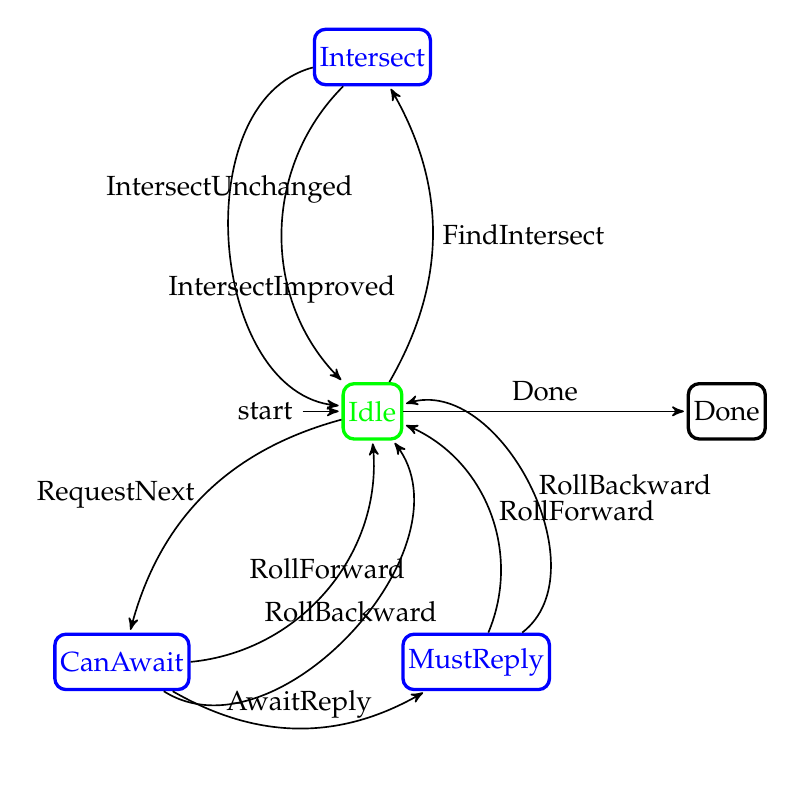
\begin{tikzpicture}[->,>=stealth',shorten >=1pt,auto,node distance=4.5cm, semithick]
  \tikzstyle{every state}=[fill=red,draw=none,text=white]
  \node[state, green, initial]                                   (Idle)      {Idle};
  \node[state, right of=Idle]                             (Done)      {Done};
  \node[state, blue, below left of=Idle]                        (CanAwait)  {CanAwait};
  \node[state, blue, right of=CanAwait]                         (MustReply) {MustReply};
  \node[state, blue, above of=Idle]                        (Intersect) {Intersect};

%  MsgRequestNext :: ChainSyncMessage header point StIdle (StNext StCanAwait)
  \draw (Idle)         edge[left, bend right]      node{RequestNext}           (CanAwait);

%  MsgAwaitReply :: ChainSyncMessage header point (StNext StCanAwait) (StNext StMustReply)
  \draw (CanAwait)     edge[above, bend right]     node{AwaitReply}            (MustReply);

%  MsgRollForward :: header -> point -> ChainSyncMessage header point (StNext any) StIdle
  \draw (CanAwait)     edge[above,bend right=45]     node{RollForward}           (Idle);
  \draw (MustReply)    edge[right,bend right=45]     node{RollForward}           (Idle);

%  MsgRollBackward :: point  -> point -> ChainSyncMessage header point (StNext any) StIdle
  \draw (CanAwait)     edge[above,bend right=80]     node{RollBackward}          (Idle);
  \draw (MustReply)    edge[right,bend right=80]     node{RollBackward}          (Idle);

%  MsgFindIntersect :: [point] -> ChainSyncMessage header point StIdle StIntersect
  \draw (Idle)         edge[right, bend right]    node{FindIntersect}         (Intersect);

%  MsgIntersectImproved  :: point -> point -> ChainSyncMessage header point StIntersect StIdle
  \draw (Intersect)    edge[above, bend right=45]    node[below = 4mm]{IntersectImproved}     (Idle);

%  MsgIntersectUnchanged :: point -> ChainSyncMessage header point StIntersect StIdle
  \draw (Intersect)    edge[above, bend right=80]    node[above = 4mm]{IntersectUnchanged}    (Idle);

%  MsgDone :: ChainSyncMessage header point StIdle StDone
  \draw (Idle)         edge[above]                node{Done}                  (Done);

\end{tikzpicture}
\end{figure}


\section{Chain Following Protocol}
\section{Block Retrieval Protocol}
\section{What other Protocols ?}
\section{Peer Discovery}
\section{Abstract and concrete representation}
\label{CBOR-section}
\begin{itemize}
  \item IER - Information Exchange Requirement
  \item CBOR - https://tools.ietf.org/html/rfc7049
\end{itemize}

\begin{itemize}
  \item CBOR as the concrete representation for the information exchanges
  \item Haskell to CBOR 
\end{itemize}

\chapter{Haskell}
While the network protocol itself can be implemented in many programming languages,
it has been developed in parallel with the Haskell reference implementation.
In addition to the language agnostic protocol decription in the other parts of this document,
this section discusses key aspects of the Haskell implementation.
This section is most useful for people who work with the Haskell reference implementation and
may give some extra insights for anybody who is interested in implementing the network.
For understanding the protocol, it is save to skip this section.
\begin{figure}
\pgfdeclareimage[height=10cm]{node-diagram-concurency}{node-diagram-concurency.pdf}
\begin{center}
\pgfuseimage{node-diagram-concurency}
\end{center}
\caption{Dataflow within a node.}
\label{node-diagram-concurency}
\end{figure}
\section{Constant Memory Consumption}
\section{The State-Machine-Framework}
\label{Haskell-state-machine}

\chapter{Discussion}
Alternative view: Exploratory work.
The real work goes here
The Why is at least as important as the What.
\section{Overview}
\section{Design Discussion}
\subsubsection{Why distinguish between node to node and node-to-consumer IPC}
\label{why_distinguish_protocols}
We use two different sets of protocols for the these two use cases.

\begin{description}
\item[node-to-node] IPC beween nodes that are engaged in the high level Ouroboros
      blockchain consensus protocol.
\item[node-to-consumer] IPC between a Cardano node and a `chain consumer' component such as a
      wallet, explorer or other custom application.
\end{description}

This section describes the differences between those two variants of IPC and why both use
different protocols.

The node-to-node protocol is conducted in a P2P environment
with very limited trust between peers. The node-to-node protocol utilises
store-and-forward over selected \emph{bearers} which form the underlying
connectivity graph. A concern in this setting is asymmetric resource consumption
attacks. Ease of implementation is a nice to have, but is subordinate to the
other hard constraints.

A node-to-consumer protocol is intended to support blockchain applications
like wallets and explorers, or Cardano-specific caches or proxies. The setting
here is that a consumer trusts a node (a `chain producer') and just wants to
catch up and keep up with the blockchain of that producer. It is assumed that
a consumer only consumes from one producer (or one of a related set of
producers), so unlike in the node-to-node protocol there is no need to choose
between different available chains. The producer may still not fully trust the
consumer and does not want to be subject to highly asymmetric resource
consumption attacks. In this use case, because of the wider range of
applications that wish to consume the blockchain, having some options that are
easy to implement is more important, even if this involves a trade-off with
performance. That said, there are also use cases where tight integration is
possible and making the most efficient use of resources is more desirable.

There are a number of applications that simply want to consume the blockchain,
but are able to rely on an upstream trusted or semi-trusted Cardano consensus
node. These applications do not need to engage in the full consensus protocol,
and may be happy to delegate the necessary chain validation.

Examples include 3rd party applications that want to observe the blockchain,
examples being business processes triggered by transactions or analytics.  It
may also include certain kinds of light client that wish to follow the
blockchain but not do full validation.

Once one considers a node-to-consumer protocol as a first class citizen then it
opens up opportunities for different system architecture choices.
The architecture of the original Cardano Mainnet release was entirely homogeneous:
every node behaved the same, each trusted nothing but itself and paid the full
networking and processing cost of engaging in the consensus protocol.  In
particular everything was integrated into a single process: the consensus
algorithm itself, serving data to other peers and components such as the wallet
or explorer. If we were to have a robust and efficient node-to-consumer protocol
then we can make many other choices.

With an efficient \emph{local} IPC protocol we can have applications
like wallets and explorers as separate processes. Even for tightly
integrated components it can make sense to run them in separate OS
processes and the associated OS mamagement tools. Not only is the
timing constraints for a consensus node are much easier to manage when
it does not have to share CPU resources with chain consumers, but it
enables the use of operating system features to give finer control
over resource consumption for sophisticated end-users.  There have
been cases in production where a highly loaded wallet component takes
more than its allowed allocation of CPU resources and causes the local
node to miss its deadlines.  By giving a consensus node a dedicated
CPU core it becomes more plausible to provide the necessary hard real
time guarantees. In addition, scaling on multi-core machines is
significantly easier with multiple OS processes than with a
multi-threaded OS process with a shared-heap. This could allow for
larger capacity Cardano relay deployments where there are multiple
network facing proxy processes that all get their chain from a single
local consensus node.

With an efficient \emph{network} IPC protocol we can do similar things
but extend it across multiple machines. This permits: large
organisations to achieve better alignment with their security
policies; clusters of relays operated by a single organisation to use
the more efficient (less resource costly) node-to-consumer protocol
instead of the node-to-node protocol; Similarly it allows for wallet
or explorer-like applications that need to scale out, and are able to
make use of a trusted node.

\section{Requirements}
\section{Threat Vectors}
\subsubsection{Asymptotic Resource consumption}
\section{Results from Simulations}
\section{Pub Sub}
\section{Of the Shelf Protocols}
\section{Meta Requirements}
\subparagraph{Work in Progress}
This document is evolved in parallel with the work on the protocol design and
the reference implementation.

\subparagraph{The Document should be Comprehensive}
\begin{itemize}
\item Top down approach.
\item Provide the big picture.
\item Usable as a reference point for a broader discussion.
\item Cover every aspect that is related to network connections.
\item Every aspect should at least have a place in the table of contents.
  If there are holes and parts that are not covered the document should say what is missing.
\item Stand alone readable with links to where missing pieces can be found.
\end{itemize}

\subparagraph{Detailed}
\begin{itemize}
\item Sufficient details to allow for new independent implementations that are compatible with
the reference implementation
\item Language agnostic (it is save to skip the Haskell specific parts)
\item Design discussions
\end{itemize}
\subparagraph{Structured}
\begin{itemize}
\item Parts of the document should be in a logical connection
\end{itemize}
\subparagraph{Workflow}

\bibliographystyle{apalike}
\bibliography{references}

\appendix
\section{Nomencenture}
\begin{description}
\item[Adversry / Adversarial Action] acting in way to subvert the
  correct (or performant) operation of the distributed protocol. Note
  that non-performance of certain functions at appropriate times can
  fall into this category.
\item[Core DIF] The set of end points that belong to the (major)
  stakepools; (the term DIF taken from RINA\ref{RINA} where it denotes
  a (potentially closed) set of potential participants.
  

\end{description}

\end{document}
